\chapter{Estado de la cuestión}
\label{chapter:estado-cuestion}

\begin{center}
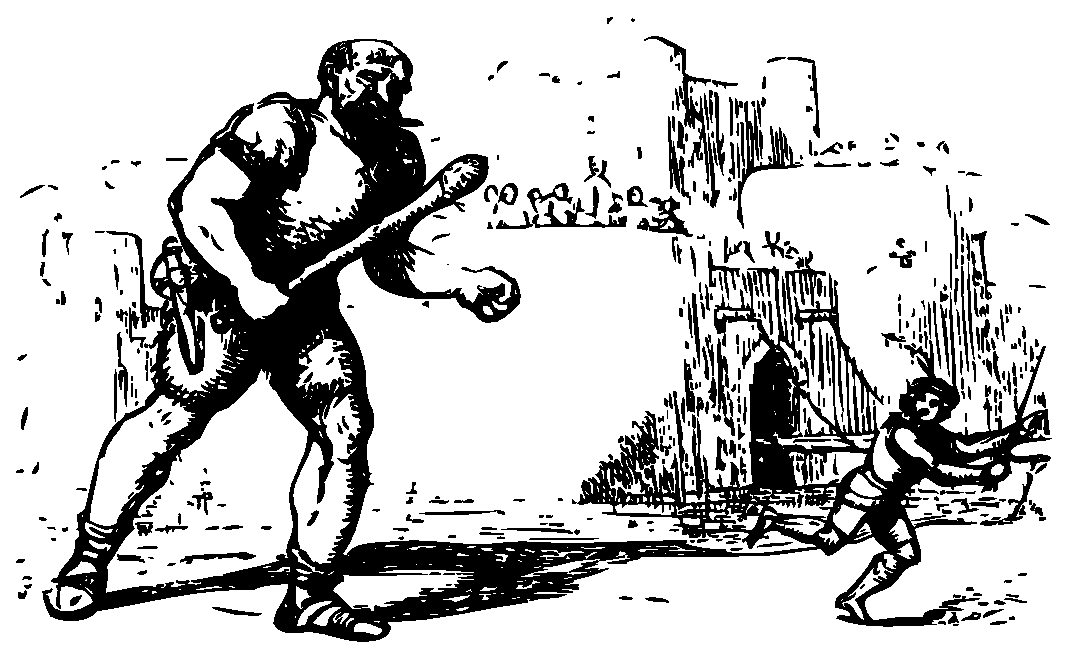
\includegraphics[scale=0.4]{../graphics/johnny_automatic_Giant_chases_Jack.eps}
\end{center}

\lettrine{E}{ste capítulo} tratará de explicar qué es el proyecto \alma{} y cuáles son sus motivaciones principales. De esta manera podemos hacernos una idea aproximada de las necesidades a cumplimentar y en qué áreas dirigir los esfuerzos. Sobre los pilares de conocimiento que se construyan aquí surgirán los demás capítulos que tratarán de dar forma a las ideas expuestas.

\section{¿Qué es el proyecto ALMA?}

En la introducción de este \pfc{} en el capítulo anterior \sectionref{introduccion} se ha comentado que uno de los sectores que todavía está en plena fase de adaptación a las nuevas tecnologías es el sector educativo. Eduardo Punset en su libro \work{Excusas para no pensar} señala que en la actualidad hay una crisis educativa y que hay que cambiar, de alguna forma, el modelo vigente \cite[No todos los niños son iguales, pág.~50]{libro:excusas-para-no-pensar}:

\begin{quotation}
\small{Curtis W. Johnson, presidente de Citistates Group y socio director de Education Evolving [\ldots], me contó que uno de los grandes errores de este sistema educativo imperante es que \guillemotleft tratamos a los niños como si fueran iguales. Los educamos igual a todos, les presentamos el material del mismo modo, y esperamos que todos aprendan las mismas cosas de la misma manera, durante el mismo día y al mismo tiempo. Esta postura no es realista, puesto que no contempla lo diferente que son los niños en muchísimas cosas, por ejemplo en el estilo de aprendizaje, pero también en el ritmo de adquisición de los conocimientos.\guillemotright{} Johnson reivindica, además, la necesidad de enseñar nuevas competencias y habilidades para que los niños y las niñas de hoy en día dominen estas técnicas para conseguir trabajo en el mundo actual. \guillemotleft La mayoría de los niños, igual que la mayoría de los jóvenes, deberán adquirir destrezas que las generaciones anteriores no tenían. Me refiero a que no solamente tendrán que aprender asignaturas básicas, sino que deberán saber cómo encontrar las cosas que necesitan saber, y luego tendrán que aprender a trabajar tal como trabaja el mundo hoy, que es principalmente en equipo [\ldots] deberán practicar el arte de la colaboración, que me parece que es el reto de colaborar con desconocidos. A todos nos encanta la idea de colaborar con nuestros amigos, y lo hacemos de muchas maneras todo el rato, pero el mundo laboral nos fuerza a llevarnos bien productivamente y crear algo de valor con gente que quizá ni siquiera nos gusta, lo cual requiere un tipo completamente distinto de educación.\guillemotright{}}
\end{quotation}

Del fragmento anterior podemos extraer las siguientes conclusiones: por un lado necesitamos hacer que la educación sea completamente personalizada, donde se adapte a las necesidades de cada persona; por otro, necesitamos centrar los esfuerzos en buscar un modelo cooperativo en los que puedan surgir las bases del aprendizaje social que es la clave que sustenta la reivindicación propuesta por Eduardo Punset y Curtis W. Johnson. Pero\ldots{} ¿qué entendemos nosotros por aprendizaje social?, ¿cómo y cuándo se produce? Esto queda explicado de manera desarrollada en \cite[pág.~1]{paper:aprendizaje-social}:

\begin{quotation}
\small{Las aulas no son los únicos entornos donde los seres humanos aprendemos, somos capaces de hacerlo en otros muchos contextos. Pensemos en cualquier escena de la vida cotidiana. Si lo hacemos descubriremos entornos no formales de desarrollo, de aprendizaje, que a menudo resultan desapercibidos. Una vez recuperada esta perspectiva de los procesos de enseñanza y aprendizaje, podemos plantearnos qué significa esta dimensión. 

Por aprendizaje social entendemos aquél aprendizaje que tiene en cuenta las interacciones sociales, es, por tanto, la forma en que los individuos adquieren conocimientos a través de la socialización e interacción con el medio.

Las teorías del aprendizaje social tienen en cuenta las interacciones sociales, pero adoptan una perspectiva de naturaleza psicológica. Destacan las relaciones entre personas que intervienen en la imitación y el modelado, y que, en consecuencia, se centran en el estudio de procesos cognitivos por los que la observación se puede convertir en fuente de aprendizaje.}
\end{quotation}


En el fragmento de arriba se menciona que el aprendizaje social \textit{requiere} de las interacciones sociales \textit{a través} de un medio en el cual los participantes pueden aprender \textit{observando}. Es innegable que una buena parte del aprendizaje, del desarrollo y de la creación de nuevas conductas en una persona tiene que ver con los factores sociales de su entorno y, no sólo eso, sino de las consecuencias positivas que le conlleva el realizar un acto que está bien visto ---bien sea por la sociedad o por los semejantes--- y que le es provechoso. Es probable que una persona que esté aprendiendo decida imitar y tomar como modelo las conductas que sean buenas ---las que se \q{premian}--- y que tienda a rechazar las que no lo son ---las que se \q{castigan}--- \cite{web:social-learning}.

Las interacciones sociales se manifiestan de múltiples maneras y formas, puesto que muchas veces su frontera no está claramente diferenciada. Podemos decir de manera análoga lo mismo para el medio. Por ejemplo, en una conversación donde intervienen dos personas, un interlocutor y un oyente (y donde es frecuente el intercambio de roles), puede ser un buen ejemplo de interacción social. El medio en este caso podría ser la voz de los participantes.
Otro ejemplo podría ser las comunicaciones indirectas en los que los individuos no interactúan en persona (\textit{chat}, teléfono, correo electrónico\ldots) y en los que el medio cobra mayor importancia, pues, condiciona la manera de recibir el mensaje. Lo que es común a ambos ejemplos es que, independientemente del medio, puede suceder que se den los mecanismos adecuados para que los individuos se enriquezcan con las aportaciones realizadas por cada participante en la conversación. Y es ahí, por lo tanto, donde se gestan las bases del aprendizaje social mencionado en el fragmento de arriba.

En la actualidad las nuevas tecnologías han creado y/o expandido nuevas formas de comunicación añadiendo o mejorando los medios existentes para expresar un mensaje. Esta última década ha supuesto un gran avance en la manera que tenemos de consumir y procesar la información. La revolución de la llamada \textit{Web 2.0} \cite{paper:innovamos} ha traído consigo una nueva forma de entender las relaciones humanas. Actualmente propuestas tan conocidas como pueden ser \textit{Flickr} \cite{web:flickr} ---donde los usuarios comparten sus fotos y votan las de los demás---, \textit{Twitter} \cite{web:twitter} ---donde los usuarios escriben en 140 caracteres lo que piensan--- o \textit{Facebook} \cite{web:facebook} ---donde el usuario tiene la posibilidad de crear un espacio virtual y tener a sus amigos cercanos en contacto--- no hacen más que reforzar el hecho de que lo social está en auge. Todos estos servicios web tienen en común la pretensión de que el usuario participe con sus semejantes de una manera cooperativa para la construcción de un conocimiento más amplio y enriquecedor.

Cabe entonces preguntarnos: ¿podemos de alguna manera aprovecharnos de las nuevas formas de interacción social y tratar de aplicarlas a un entorno de enseñanza y aprendizaje que pueda ser cooperativo? La respuesta es que si y es en esta linea en la que trabaja el proyecto \alma{}. 

La misión principal de éste es que trata de crear espacios alternativos de enseñanza y aprendizaje a los que tenemos en la actualidad sin tratar de sustituirlos  ---por ejemplo, un aula tradicional donde se imparte una asignatura--- si no más bien de complementarlos. Para ello se apoya en herramientas sociales cooperativas como son las \textit{wikis}. De esta manera se logra personalizar la educación, adaptarla al ritmo de cada individuo (como señalaban Punset y Johnson anteriormente) y hacerla más social e interactiva. En el siguiente fragmento se explica de manera detallada las ventajas que aportan usar un \textit{software wiki} en un aula \cite[pág.~4]{paper:innovamos}:

\begin{quotation}
\small{¿Qué es una \textit{wiki}? Imaginemos un sitio web cooperativo donde los usuarios pudieran crear, editar, borrar o modificar el contenido. ¡Eso es una \textit{wiki}! La \textit{wiki} más conocida es la Wikipedia \cite{web:wikipedia}, una enciclopedia creada a partir de las aportaciones de todos los usuarios que la visitan.

¿Cómo podemos utilizar una \textit{wiki} en nuestras clases? Una \textit{wiki} nos permite crear un espacio de trabajo cooperativo con nuestros alumnos. Podemos montar una \textit{wiki} para editar, entre todos, los apuntes de una asignatura (\textit{wiki-apuntes}), o podemos utilizarla para crear un glosario con los términos conceptuales que surjan durante las clases. Incluso podemos proponer a los alumnos que mejoren algún artículo ya existente en la Wikipedia y que guarde relación con su asignatura, como por ejemplo este: \url{http://es.wikipedia.org/wiki/Derecho_romano}.

Son muchas las posibilidades de trabajo que acerca un espacio \textit{wiki} al proceso de enseñanza y aprendizaje de los alumnos, y como docentes debemos indagar en ellas.

Todas las ediciones y cambios que se hacen en una \textit{wiki} quedan registradas, de forma que el profesor sabe qué ha editado quien, y cuando lo ha hecho. Una \textit{wiki} permite a los alumnos y al profesor editar de una forma muy sencilla los contenidos de un sitio web. Todos pueden trabajar editando un glosario con los conceptos de la asignatura, y además establecer discusiones sobre cada concepto en el que trabaja la clase. Es por lo tanto una herramienta sencilla y que facilita enormemente la tarea de editar contenidos en grupo.

Sobre la utilización de las \textit{wikis} en la docencia podemos decir muchas más cosas. Rompen la asimetría y la unidireccionalidad de la enseñanza, de modo que los propios alumnos son los que enseñan a sus compañeros, pues el conocimiento se construye entre todos. El profesor adquiere nuevos roles: facilitador, moderador, orientador, y evaluador (continuo). También lo hacen los alumnos: colaboradores, cooperadores y capaces de enseñar a sus compañeros. Las barreras de la clase se superan de tal forma que podemos compartir y generar conocimiento con el resto del mundo.}
\end{quotation}

Como queda demostrado arriba las \textit{wikis}, por su naturaleza, se asientan en los principios de las \textit{interacciones sociales}, es decir, se nutren de las participaciones de todas las personas. Además, su máximo interés reside en el hecho de que se dispone de una total libertad para poder modificar tantas veces se quiera el \textit{mensaje} (pudiendo crear nuevos contenidos, editarlos, borrarlos y recuperarlos cuando y como deseemos). A esto es a lo que se conoce como \textit{filosofía wiki} (\figureref{filosofia_wiki}) \cite{video:wikis-plain-english}. Lo maravilloso de esta forma de trabajar es que, de manera inconsciente, se acaba creando lo que \citeauthor{libro:comunidades-de-practica-wenger-primera-edicion} en su libro \work{Communities of Practice: Learning, Meaning, and Identity} \cite{libro:comunidades-de-practica-wenger-primera-edicion} denominó por primera vez, en \citeyear{libro:comunidades-de-practica-wenger-primera-edicion}, como \textit{comunidades de práctica}. Y\ldots{} ¿qué son exactamente?

\begin{figure}
\centering
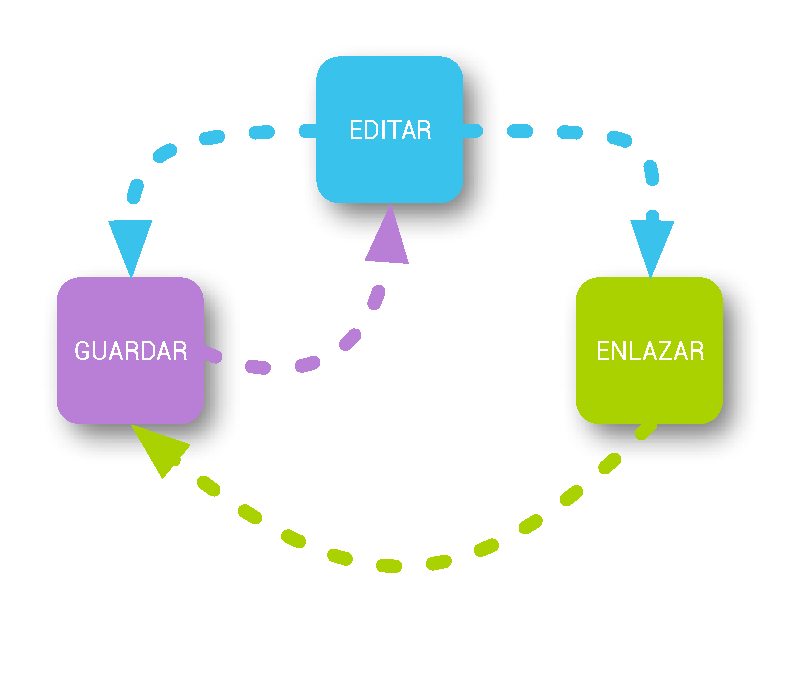
\includegraphics[width=\linewidth]{../graphics/fig_filosofia_wiki.eps}
\caption{Flujo de trabajo en la filosofía \textit{wiki}. Como podemos observar, éste se repite indefinidamente.}\label{fig:filosofia_wiki}
\end{figure}
 
Una definición, más o menos formal, podría decir que: \q{las comunidades de práctica se originan cuando existe un grupo de individuos que comparten un interés, o un conjunto de problemas o una pasión sobre un tema determinado y, que profundizan tanto su conocimiento y experiencia en el área, que lo que produce es que las relaciones entre los distintos miembros se acaban fortaleciendo} \cite{paper:filwit}.

Las comunidades de práctica se pueden dar en múltiples ámbitos (o en todos a la vez), es más, es bastante probable que cualquier persona que tenga una afición, sea cual sea, por el mero hecho de compartir sus gustos con otras personas ésta pertenezca ya, sin saberlo, a una comunidad de práctica. Aunque hay que discernir que no todas las comunidades a las que se puede pertenecer son comunidades de práctica. Para que lo sean se deben dar tres características fundamentales:

\begin{itemize}
\item \textit{Dominio}: es el campo de interés compartido por la comunidad y es el que crea una identidad común al grupo.

\item \textit{Comunidad}: es aquí donde los miembros establecen las relaciones que les permiten aprender y, a su vez, exponer su experiencia y su conocimiento en un tema determinado.

\item \textit{Práctica}: los miembros forman parte del proceso mismo, participando en actividades de manera conjunta y donde se comparten los intereses de la comunidad.
\end{itemize}

Como las comunidades de práctica se pueden dar en cualquier lugar es por eso que se mencionaba anteriormente que el \textit{software wiki} las genera de manera inconsciente. Si lo pensamos bien, podemos llegar a la siguiente conclusión: el \textit{software wiki} es utilizado de tal manera que es un \textit{medio} que sirve como causa para lograr un \textit{fin} que no es otro que el \textit{dominio}, la \textit{comunidad} y la \textit{práctica}. (En la \figureref{comunidades_de_practica} podemos ver a diferentes comunidades de práctica trabajando en grupos y que están implementadas sobre una plataforma \textit{wiki} cualquiera.)

\begin{figure}
\centering
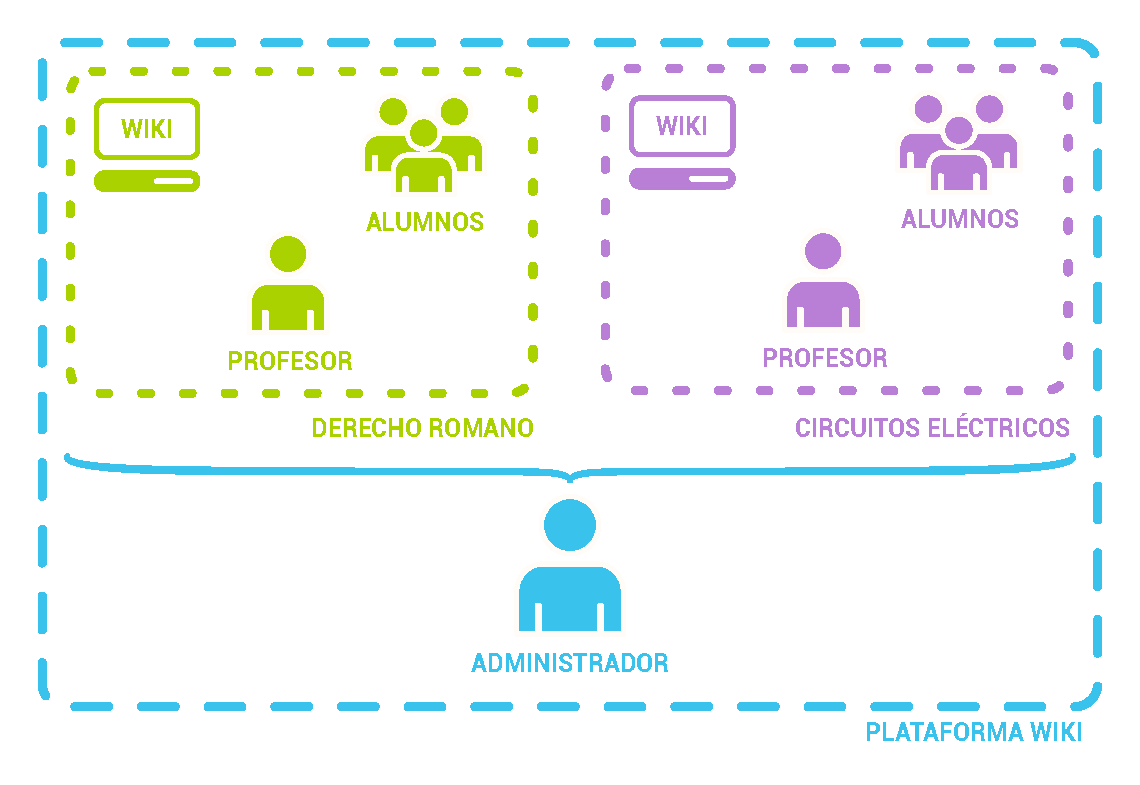
\includegraphics[width=\linewidth]{../graphics/fig_comunidades_de_practica.eps}
\caption{Distintas comunidades de práctica trabajando conjuntamente en su propio dominio. El administrador de la plataforma es el encargado de que todo funcione correctamente.}\label{fig:comunidades_de_practica}
\end{figure}

Otro aspecto importante que hay que tener en cuenta y que se puede ver analizando la \figureref{comunidades_de_practica}, son los roles y las interacciones que se producen en una comunidad de práctica. \citeauthor{libro:comunidades-de-practica-wenger} en el libro \work{Cultivating Communities of Practice: A Guide to Managing Knowledge} \cite{libro:comunidades-de-practica-wenger} sostienen que no sólo es significativo pensar en las tres características que conforman las comunidades de práctica, sino que hay que dar un paso adelante y analizar los diferentes perfiles que hay dentro de ellas. Esto se debe a que no todos los miembros de una comunidad de práctica participan en ésta de forma equitativa; cada persona tiene un nivel distinto de interés en el papel que le toca desempeñar. Estos son los diferentes roles o niveles de participación que podemos encontrar (clasificados de menor a mayor grado de implicación):

\begin{itemize}

\item \textit{Agentes externos}: No pertenecen directamente a la comunidad pero muestran una inclinación en ésta, puede ser que como clientes o porque comparten algún punto de interés.

\item \textit{Miembros periféricos}: Este grupo pertenece a la comunidad y su característica principal es que participan en escasas ocasiones y son el grupo mayoritario. Normalmente suelen observar las interacciones de los miembros activos, del núcleo y de los coordinadores. Las motivaciones del porqué no participan suelen ser porque consideran que sus aportaciones no son importantes para la comunidad o que no poseen con la autoridad suficiente para que sean tenidos en cuenta. Otros, en cambio, consideran simplemente que no quieren participar porque no disponen de tiempo suficiente para ser más activos. Aún así, sus actividades periféricas, son sumamente importantes para el resto ya que gracias a su observación de todo lo que sucede dentro, consiguen obtener una visión amplia de todo lo que se expone.

\item \textit{Miembros activos}: Este grupo son aquellos que, según Wenger y col., suelen participar ocasionalmente en los foros u otras actividades de la comunidad pero sin llegar al nivel de intensidad de los miembros del núcleo. No suele ser un grupo muy amplio, ya que quizá no llegue a más del 15 ó 20\% de la comunidad.

\item \textit{Núcleo}: Es, por lo general, el grupo más compacto y pequeño que participa activamente en todas las actividades de la comunidad de una forma activa. Son los que guían a la comunidad a través de una agenda de actividades. Conforme la comunidad va madurando, este grupo suele tomar una buena parte del liderazgo junto con el coordinador. Es un grupo minoritario que no comprende más del 10\% de los participantes.

\item \textit{Coordinador}: Es el encargado de organizar eventos y conectar a los diferentes miembros de la comunidad. Su contribución se basa en que la comunidad esté enfocada en su dominio, que mantenga relaciones entre sus miembros y otras comunidades, y que desarrolle su práctica. La dedicación de esta persona como coordinador es bastante alta, típicamente los valores oscilan entre 20 y el 50\% de su tiempo. Además, sus otras funciones principales son:
\begin{itemize}
\item Vela por que la comunidad esté siempre activa y que se produzcan contribuciones de ésta a los demás miembros.
\item Relaciona informalmente miembros de la comunidad.
\item Planea y facilita eventos en la comunidad.
\item Contribuye en la construcción de la práctica. Esto incluye trabajar en la administración del conocimiento en la comunidad, lecciones aprendidas, mejores prácticas y métodos para el aprendizaje.
\item Identifica cuestiones o temas importantes en el dominio de la comunidad.
\item Posee una buena relación con el Núcleo y distribuye ciertas tareas con dicho grupo.
\end{itemize}
\end{itemize}

Saber identificar estos roles nos ayuda a entender como funcionan las comunidades de práctica internamente. También nos da una idea general de que características necesita una plataforma \textit{wiki} para que la implementación sea lo más afín a la definición dada.

Por lo tanto, en el siguiente capítulo nos veremos en la necesidad de buscar un \textit{software} que pueda implementar de manera fiable todo lo que aquí se ha explicado ya que la clave que sustenta al proyecto \alma{}, son al fin y al cabo, las comunidades de práctica.